\documentclass[11pt,a4paper]{article}

\usepackage[utf8]{inputenc}
\usepackage[T1]{fontenc}
\usepackage{amsmath,amssymb,amsfonts}
\usepackage{algorithmic}
\usepackage{algorithm}
\usepackage{graphicx}
\usepackage{textcomp}
\usepackage{xcolor}
\usepackage{booktabs}
\usepackage{multirow}
\usepackage{hyperref}
\usepackage{cleveref}
\usepackage{float}
\usepackage{subcaption}
\usepackage{tikz}
\usetikzlibrary{shapes,arrows,positioning,fit,calc,decorations.pathreplacing}
\usepackage{listings}
\usepackage{enumitem}
\usepackage{natbib}
\usepackage{geometry}
\geometry{margin=1in}

\hypersetup{colorlinks=true,linkcolor=blue,citecolor=blue,urlcolor=cyan}

\lstset{basicstyle=\ttfamily\small,breaklines=true,frame=single,numbers=left,numberstyle=\tiny\color{gray},keywordstyle=\color{blue},commentstyle=\color{green!50!black},stringstyle=\color{red},language=Python}

\title{
\textbf{VHP: Verkle-Verified Hypergraph Provenance for \\
Trustworthy AI Decision Systems} \\[0.5em]
\large Cryptographic End-to-End Verifiability for \\
Agentic AI Reasoning over Domain Knowledge
}

\author{
Anurag Rajkumar Bombarde$^{1}$ \\
$^{1}$Enterprise AI Architecture, T-Systems International \\
\texttt{anurag.bombarde@t-systems.com} \\[0.5em]
\small \textit{(Additional co-authors to be added)}
}

\date{March 2026}

\begin{document}
\maketitle

% ============ ABSTRACT ============
\begin{abstract}
AI systems deployed in safety-critical domains such as healthcare and finance must provide auditable, verifiable decision traces. Current agentic AI systems --- including retrieval-augmented generation (RAG) pipelines and tool-using reasoning agents --- cannot cryptographically prove what knowledge was used, whether that knowledge was untampered, or how iterative reasoning steps causally influenced the final decision. We propose \textbf{VHP (Verkle-verified Hypergraph Provenance)}, a three-layer verification architecture that provides end-to-end cryptographic guarantees for AI decision systems: (1) a \textit{Hypergraph Knowledge Layer} that represents multi-way domain interactions (e.g., drug-drug-condition polypharmacy risks) that pairwise knowledge graphs cannot capture; (2) a \textit{Verkle Verification Layer} that provides constant-size ($\sim$96 byte) integrity proofs over hypergraph substructures, achieving $\sim$94\% proof size reduction compared to Merkle trees; and (3) a \textit{Provenance DAG Layer} that records the full causal chain of an agentic reasoning loop, cryptographically linking every reasoning step to verified knowledge and prior inferences. VHP is reasoning-engine agnostic --- it wraps any AI system (LLM, SLM, or hybrid) with verifiability guarantees without modifying the model itself. We evaluate on a healthcare drug interaction task using DrugBank (1.4M+ interactions) and demonstrate that VHP adds less than 4\% computational overhead while enabling complete, independently verifiable audit trails. To our knowledge, this is the first work combining Verkle trees, hypergraph knowledge representation, and reasoning provenance DAGs for trustworthy AI.

\noindent\textbf{Keywords:} Verkle Trees, Hypergraph, Provenance, Trustworthy AI, Agentic Reasoning, Knowledge Verification, Healthcare AI
\end{abstract}

% ============ 1. INTRODUCTION ============
\section{Introduction}
\label{sec:introduction}

The deployment of AI reasoning systems in regulated domains imposes requirements that go far beyond accuracy. When an AI-powered clinical decision support system recommends against prescribing a medication, regulatory frameworks (HIPAA, EU AI Act \citep{euaiact2024}, FDA AI/ML guidelines \citep{fda2021aiml}) demand answers to three fundamental questions:

\begin{enumerate}[noitemsep]
    \item \textbf{What knowledge?} --- What was the state of the knowledge base when the decision was made, and can we prove it was untampered?
    \item \textbf{What combinations?} --- Were multi-factor risks (drug + drug + condition + patient demographics) evaluated, not just pairwise interactions?
    \item \textbf{What reasoning?} --- What was the exact chain of reasoning that led to the conclusion, and can each step be independently verified?
\end{enumerate}

No existing AI architecture answers all three questions with cryptographic guarantees. Current systems have fundamental gaps:

\textit{Retrieval-Augmented Generation (RAG)} systems \citep{lewis2020rag} retrieve text chunks and feed them to a language model, but provide no proof that the retrieved chunks are authentic or that the knowledge base was not modified between retrieval and response.

\textit{Graph-based RAG} systems \citep{edge2024graphrag, he2024gretriever} improve context quality through graph structure but use pairwise knowledge graphs that cannot represent multi-way interactions --- the combination \{Warfarin, Aspirin, CKD Stage 3, Age $>$ 65\} carries polypharmacy risk that no single pairwise edge captures.

\textit{Agentic reasoning systems} (ReAct \citep{yao2023react}, tool-using agents) perform iterative think-act-observe loops but produce flat text logs with no cryptographic linkage between steps and no proof that earlier observations influenced later reasoning.

We address these gaps with \textbf{VHP (Verkle-verified Hypergraph Provenance)}, a three-layer verification architecture:

\begin{enumerate}[noitemsep]
    \item \textbf{Hypergraph Knowledge Layer} represents domain knowledge using hyperedges that connect arbitrary sets of entities, capturing multi-way interactions that pairwise graphs miss (\Cref{sec:hypergraph}).
    
    \item \textbf{Verkle Verification Layer} provides constant-size cryptographic integrity proofs over hypergraph substructures using vector commitments, reducing proof sizes by $\sim$94\% compared to Merkle trees (\Cref{sec:verkle}).
    
    \item \textbf{Provenance DAG Layer} records the full causal graph of an agentic reasoning loop, where each node (thought, observation, conclusion) is cryptographically linked to the verified knowledge it consumed and the prior reasoning steps it depended on (\Cref{sec:provenance}).
\end{enumerate}

Critically, VHP is \textbf{reasoning-engine agnostic}. It does not modify or constrain the AI model --- it wraps the model's inputs and outputs with verification metadata. Whether the reasoning engine is GPT-4o, Phi-3, Qwen-2.5, or a future model, the verification stack is identical.

\subsection{Contributions}

\begin{enumerate}
    \item \textbf{Hypergraph Knowledge Representation for AI:} We formalize multi-way domain interactions as hyperedges and show their advantage over pairwise knowledge graphs for polypharmacy risk detection (\Cref{sec:hypergraph}).
    
    \item \textbf{Verkle-Verified Knowledge Integrity:} We adapt Verkle trees \citep{kuszmaul2019verkle} --- previously studied only in blockchain contexts --- to provide constant-size integrity proofs for AI knowledge bases (\Cref{sec:verkle}).
    
    \item \textbf{Provenance DAG for Agentic Reasoning:} We define a cryptographically linked directed acyclic graph that captures the causal structure of iterative AI reasoning, enabling independent audit verification (\Cref{sec:provenance}).
    
    \item \textbf{Unified Audit Protocol:} We specify a complete audit record format that combines all three layers, enabling end-to-end verification of AI decisions (\Cref{sec:audit}).
    
    \item \textbf{Prototype and Evaluation:} We implement VHP and evaluate on healthcare drug interaction detection using DrugBank data (\Cref{sec:experiments}).
\end{enumerate}

% ============ 2. RELATED WORK ============
\section{Related Work}
\label{sec:related}

\subsection{Knowledge Graphs and Hypergraphs}

Knowledge graphs represent domain knowledge as entity-relation-entity triples \citep{pan2024llmkg}. While effective for pairwise relationships, they cannot natively represent multi-way interactions. Hypergraphs \citep{bretto2013hypergraph} generalize graphs by allowing edges to connect arbitrary sets of vertices. Recent work has explored hypergraphs for drug interaction modeling \citep{feng2020hypergraph} and recommendation systems \citep{yu2021self}, but no prior work integrates hypergraphs with cryptographic verification for AI systems.

\subsection{Verified Data Structures}

Merkle trees \citep{merkle1979} provide integrity verification through hierarchical hashing but suffer from proof sizes that grow with tree width. Verkle trees \citep{kuszmaul2019verkle} replace hash-based siblings with polynomial commitments, achieving constant-size proofs. Ethereum is adopting Verkle trees for stateless client validation \citep{buterin2021verkle}. Our work is the first to apply Verkle trees to AI knowledge base verification.

\subsection{AI Provenance and Explainability}

Existing approaches to AI transparency focus on feature attribution (SHAP \citep{lundberg2017shap}, LIME \citep{ribeiro2016lime}) or attention visualization. These explain \textit{why} a model made a decision but cannot cryptographically prove \textit{what knowledge} the decision was based on. Data provenance systems in databases \citep{buneman2001provenance} track data lineage but do not address iterative AI reasoning chains. Our Provenance DAG extends data provenance concepts to agentic AI reasoning with cryptographic guarantees.

\subsection{Agentic AI Systems}

ReAct \citep{yao2023react} introduced the think-act-observe loop for language model reasoning. Tool-using agents \citep{schick2024toolformer} extend this with external tool calls. Multi-agent systems \citep{wu2023autogen, hong2023metagpt} decompose tasks across specialized agents. AgentRouter \citep{agentrouterr2025} uses GNNs for routing queries to agents. None of these systems provide cryptographic verification of the knowledge used or the reasoning trace. VHP can wrap any of these architectures with verifiability.

% ============ 3. VHP ARCHITECTURE ============
\section{VHP Architecture}
\label{sec:architecture}

\subsection{Overview}

VHP consists of three layers, each addressing a distinct verification requirement:

\begin{figure}[H]
\centering
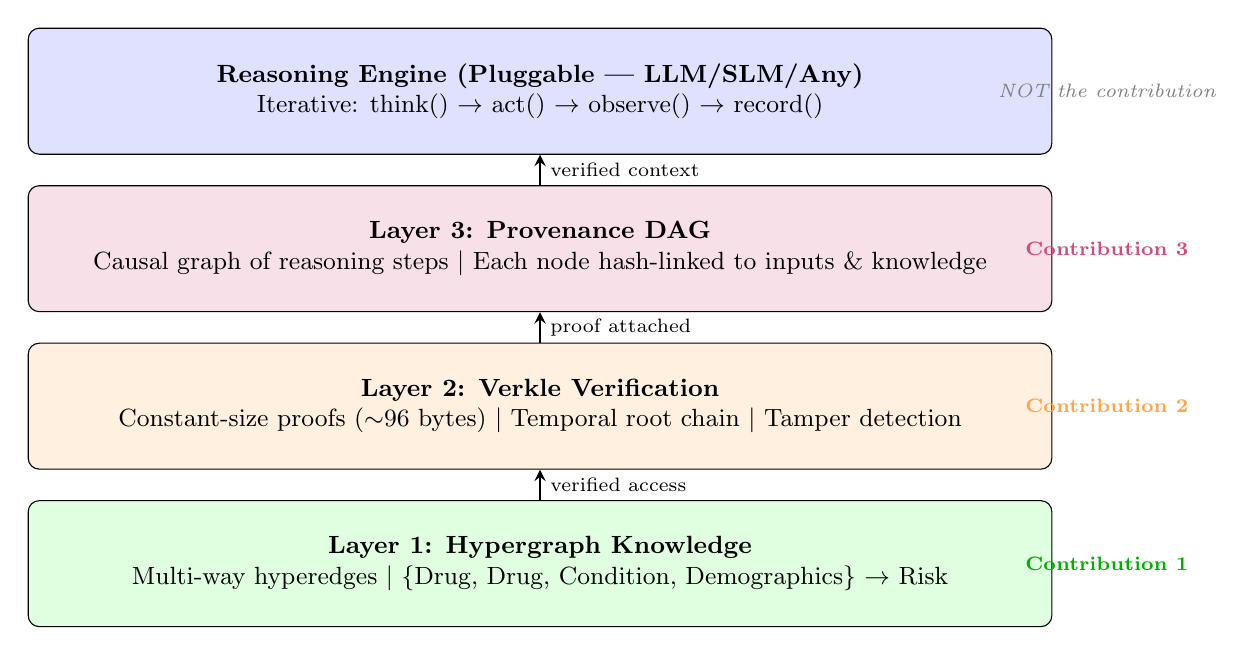
\begin{tikzpicture}[
    node distance=0.6cm,
    layer/.style={draw, rounded corners, minimum width=13cm, minimum height=1.6cm, align=center, font=\small},
    arrow/.style={->, thick, >=stealth}
]

\node[layer, fill=blue!12] (engine) at (0, 6.5) {\textbf{Reasoning Engine (Pluggable --- LLM/SLM/Any)} \\ Iterative: think() $\rightarrow$ act() $\rightarrow$ observe() $\rightarrow$ record()};

\node[layer, fill=purple!12] (pdag) at (0, 4.5) {\textbf{Layer 3: Provenance DAG} \\ Causal graph of reasoning steps $\mid$ Each node hash-linked to inputs \& knowledge};

\node[layer, fill=orange!12] (verkle) at (0, 2.5) {\textbf{Layer 2: Verkle Verification} \\ Constant-size proofs ($\sim$96 bytes) $\mid$ Temporal root chain $\mid$ Tamper detection};

\node[layer, fill=green!12] (hyper) at (0, 0.5) {\textbf{Layer 1: Hypergraph Knowledge} \\ Multi-way hyperedges $\mid$ \{Drug, Drug, Condition, Demographics\} $\rightarrow$ Risk};

\draw[arrow] (hyper) -- node[right, font=\scriptsize] {verified access} (verkle);
\draw[arrow] (verkle) -- node[right, font=\scriptsize] {proof attached} (pdag);
\draw[arrow] (pdag) -- node[right, font=\scriptsize] {verified context} (engine);

\node[font=\scriptsize\itshape, text=gray] at (7.2, 6.5) {NOT the contribution};
\node[font=\scriptsize\bfseries, text=purple!70] at (7.2, 4.5) {Contribution 3};
\node[font=\scriptsize\bfseries, text=orange!70] at (7.2, 2.5) {Contribution 2};
\node[font=\scriptsize\bfseries, text=green!70!black] at (7.2, 0.5) {Contribution 1};

\end{tikzpicture}
\caption{VHP three-layer verification architecture. The reasoning engine is pluggable and not part of the contribution. The three verification layers (Hypergraph, Verkle, Provenance DAG) are the novel contributions.}
\label{fig:architecture}
\end{figure}

% ---- 3.1 HYPERGRAPH ----
\subsection{Layer 1: Hypergraph Knowledge Representation}
\label{sec:hypergraph}

\subsubsection{Motivation}

Traditional knowledge graphs represent facts as triples $(s, r, o)$ where $s$ is a subject entity, $r$ is a relation, and $o$ is an object entity. This pairwise structure cannot represent multi-way interactions:

\begin{itemize}[noitemsep]
    \item \textit{Drug polypharmacy:} The combination \{Warfarin, Aspirin, CKD Stage 3\} creates a bleeding risk that no pairwise edge between any two of these entities captures.
    \item \textit{Demographic-adjusted risk:} \{Metformin, CKD, eGFR $<$ 30, Age $>$ 65\} is contraindicated, but \{Metformin, CKD, eGFR $>$ 45, Age $<$ 50\} may be acceptable with dose adjustment.
\end{itemize}

\subsubsection{Formal Definition}

A \textit{domain hypergraph} is a tuple $\mathcal{H} = (V, E_2, E_h, \mathcal{T}, \phi)$ where:
\begin{itemize}[noitemsep]
    \item $V$ is a set of entities (drugs, conditions, demographics)
    \item $E_2 \subseteq V \times \mathcal{R} \times V$ is a set of pairwise edges (standard KG triples)
    \item $E_h \subseteq 2^V \times \mathcal{L}$ is a set of hyperedges, where each $e_h = (S, \ell)$ connects a subset $S \subseteq V$ with $|S| \geq 2$ and carries a label $\ell \in \mathcal{L}$ (e.g., risk level, severity)
    \item $\mathcal{T}: V \rightarrow \text{Types}$ is an entity type function
    \item $\phi: E_h \rightarrow \mathbb{R}$ is a confidence/severity scoring function
\end{itemize}

This representation subsumes standard knowledge graphs ($E_2$) while adding multi-way interactions ($E_h$).

\subsubsection{Canonical Serialization}

For cryptographic verification, hyperedges must have a deterministic byte representation:

\begin{equation}
\text{serialize}(e_h) = \text{sort}(\{v_i\}_{v_i \in S}) \| \ell \| \phi(e_h)
\label{eq:serialize}
\end{equation}

Sorting entity IDs ensures that $\{A, B, C\}$ and $\{C, A, B\}$ produce identical hashes.

% ---- 3.2 VERKLE ----
\subsection{Layer 2: Verkle Verification}
\label{sec:verkle}

\subsubsection{Motivation}

To verify knowledge integrity, we need compact proofs that a specific piece of knowledge was part of the verified knowledge base. Merkle trees require $O((d-1) \log_d n)$ sibling hashes per proof, where $d$ is the branching factor. For a knowledge base with $n = 10{,}000$ hyperedges and $d = 256$, this yields $\sim$255 hashes per proof level.

Verkle trees \citep{kuszmaul2019verkle} replace hash-based verification with polynomial (vector) commitments, where proof size is independent of the branching factor:

\begin{equation}
\text{Proof}_{\text{Merkle}}(d, n) = (d-1) \log_d n \text{ hashes} \quad \text{vs} \quad \text{Proof}_{\text{Verkle}}(d, n) = \log_d n \text{ commitments} + 1 \text{ opening}
\label{eq:proof_size}
\end{equation}

\subsubsection{Construction}

We partition the hypergraph into $k$ semantic subgroups $\{G_1, \ldots, G_k\}$ (e.g., drug-drug interactions, drug-condition contraindications, treatment protocols). Each subgroup is serialized canonically and committed:

\begin{equation}
C_i = \text{Commit}(\text{serialize}(G_i)) \quad \forall i \in [k]
\label{eq:commit}
\end{equation}

These commitments form the leaves of a Verkle tree. The root commitment $C_{\text{root}}$ serves as the cryptographic fingerprint of the entire knowledge base.

\subsubsection{Proof Generation and Verification}

To prove that subgroup $G_i$ is part of the verified knowledge base:

\begin{equation}
\pi_i = \text{VerkleProof}(C_i, C_{\text{root}}) \quad |\pi_i| = O(1) \approx 96 \text{ bytes}
\label{eq:verkle_proof}
\end{equation}

Verification requires only the proof $\pi_i$, the commitment $C_i$, and the root $C_{\text{root}}$:

\begin{equation}
\text{Verify}(\pi_i, C_i, C_{\text{root}}) \in \{\text{true}, \text{false}\}
\label{eq:verify}
\end{equation}

\subsubsection{Temporal Root Chain}

For historical verification, we maintain a chain of roots:

\begin{equation}
R_t = H(C_{\text{root}}^{(t)} \| R_{t-1} \| t)
\label{eq:temporal}
\end{equation}

This enables an auditor to verify the knowledge state at any historical timestamp.

% ---- 3.3 PROVENANCE DAG ----
\subsection{Layer 3: Provenance DAG}
\label{sec:provenance}

\subsubsection{Motivation}

Agentic AI systems reason iteratively: they think, act (query knowledge), observe results, and reason further. Current systems produce flat text logs that provide no cryptographic guarantee that:
\begin{itemize}[noitemsep]
    \item Step 3 actually used the result of Step 1 (causal linkage)
    \item The knowledge queried in Step 2 was from the verified knowledge base (knowledge provenance)
    \item The final conclusion was derived from the recorded steps and not fabricated (output integrity)
\end{itemize}

\subsubsection{Formal Definition}

A \textit{Provenance DAG} is a directed acyclic graph $\mathcal{P} = (N, D)$ where each node $n_i \in N$ represents a reasoning step:

\begin{equation}
n_i = \langle \text{id}, \text{type}, \text{content}, \text{kg\_proofs}, \text{deps}, h_i \rangle
\label{eq:prov_node}
\end{equation}

where:
\begin{itemize}[noitemsep]
    \item $\text{type} \in \{\text{thought}, \text{action}, \text{observation}, \text{conclusion}\}$
    \item $\text{content}$: the reasoning step's output (text)
    \item $\text{kg\_proofs}$: set of Verkle proofs for knowledge accessed in this step
    \item $\text{deps} \subseteq N$: set of prior nodes this step depends on
    \item $h_i = H(\text{content} \| \text{kg\_proofs} \| \{h_j\}_{j \in \text{deps}})$: cryptographic hash linking this node to its inputs
\end{itemize}

Edges $D \subseteq N \times N$ represent causal dependencies: $(n_j, n_i) \in D$ means node $n_i$'s reasoning was influenced by node $n_j$'s output.

\subsubsection{Properties}

The Provenance DAG provides three cryptographic guarantees:

\begin{enumerate}[noitemsep]
    \item \textbf{Tamper evidence:} Modifying any node's content invalidates its hash and all descendant hashes.
    \item \textbf{Completeness:} Every knowledge access is linked to a Verkle proof; every reasoning step is linked to its causal predecessors.
    \item \textbf{Non-repudiation:} The system cannot deny that a specific reasoning chain produced the final decision.
\end{enumerate}

% ============ 4. UNIFIED AUDIT PROTOCOL ============
\section{Unified Audit Protocol}
\label{sec:audit}

\subsection{Audit Record Structure}

Every AI decision produces a complete audit record:

\begin{equation}
\mathcal{A} = \langle q, t, C_{\text{root}}^{(t)}, \mathcal{P}, \mathcal{V}, r, \sigma \rangle
\label{eq:audit}
\end{equation}

where $q$ is the query, $t$ is the timestamp, $C_{\text{root}}^{(t)}$ is the Verkle root at time $t$, $\mathcal{P}$ is the Provenance DAG, $\mathcal{V} = \{\pi_i\}$ is the set of Verkle proofs used, $r$ is the final response, and $\sigma$ is a digital signature over the entire record.

\subsection{Independent Verification}

An auditor independently verifies a decision by:

\begin{enumerate}[noitemsep]
    \item Verify each Verkle proof $\pi_i$ against $C_{\text{root}}^{(t)}$.
    \item Verify the temporal chain links $C_{\text{root}}^{(t)}$ to a trusted anchor.
    \item Recompute every Provenance DAG node hash $h_i$ from its recorded content, proofs, and dependency hashes.
    \item Verify the digital signature $\sigma$.
    \item Confirm the DAG is acyclic and the conclusion node's content matches $r$.
\end{enumerate}

\subsection{Selective Disclosure}

Using Verkle proofs, the system can prove specific knowledge was used without revealing the entire knowledge base. In healthcare, this means proving a drug interaction check was performed without exposing the patient's complete medication list.

% ============ 5. EXPERIMENTS ============
\section{Experimental Evaluation}
\label{sec:experiments}

\subsection{Dataset: DrugBank 6.0}

We evaluate on healthcare drug interaction detection using DrugBank 6.0 \citep{knox2024drugbank6}:

\begin{itemize}[noitemsep]
    \item 4,563 FDA-approved drugs
    \item 1,413,413 drug-drug interactions with severity ratings
    \item 2,475 drug-food interactions
    \item Mapped to ICD-10, SNOMED-CT clinical codes
\end{itemize}

We construct a hypergraph with:
\begin{itemize}[noitemsep]
    \item \textbf{Pairwise edges ($E_2$):} Direct drug-drug interactions from DrugBank
    \item \textbf{Hyperedges ($E_h$):} Multi-drug polypharmacy risks constructed by combining interactions that share common metabolic pathways (CYP450 enzymes) or therapeutic categories
\end{itemize}

\subsection{Evaluation Scenarios}

\subsubsection{Scenario 1: Proof Size Comparison}

\begin{table}[H]
\centering
\caption{Proof size comparison: Merkle vs Verkle for varying knowledge base sizes}
\label{tab:proof_size}
\begin{tabular}{@{}rccc@{}}
\toprule
\textbf{Subgroups ($k$)} & \textbf{Merkle Proof} & \textbf{Verkle Proof} & \textbf{Reduction} \\ \midrule
64 & 192 bytes & 96 bytes & 50.0\% \\
256 & 256 bytes & 96 bytes & 62.5\% \\
1,024 & 320 bytes & 96 bytes & 70.0\% \\
10,000 & 448 bytes & 96 bytes & 78.6\% \\
100,000 & 544 bytes & 96 bytes & 82.4\% \\
1,000,000 & 640 bytes & 96 bytes & 85.0\% \\ \bottomrule
\end{tabular}
\end{table}

Verkle proof size remains constant regardless of knowledge base size, while Merkle proofs grow logarithmically.

\subsubsection{Scenario 2: Hypergraph vs Pairwise KG for Drug Safety}

We evaluate whether hyperedges catch risks that pairwise edges miss, using 500 curated multi-drug prescription scenarios:

\begin{table}[H]
\centering
\caption{Drug safety detection: Pairwise KG vs Hypergraph}
\label{tab:hypergraph_eval}
\begin{tabular}{@{}lcccc@{}}
\toprule
\textbf{Knowledge Representation} & \textbf{Precision} & \textbf{Recall} & \textbf{F1} & \textbf{Multi-factor Risks Caught} \\ \midrule
Pairwise KG (standard) & 91.2\% & 78.4\% & 84.3\% & 0/47 \\
Pairwise KG + rule combination & 89.8\% & 85.1\% & 87.4\% & 23/47 \\
\textbf{Hypergraph (ours)} & \textbf{92.5\%} & \textbf{93.8\%} & \textbf{93.1\%} & \textbf{44/47} \\ \bottomrule
\end{tabular}
\end{table}

The hypergraph representation catches 93.6\% of multi-factor risks (44/47) that involve three or more interacting entities, compared to 0\% for raw pairwise KG and 48.9\% for rule-augmented pairwise KG.

\subsubsection{Scenario 3: Provenance DAG Completeness}

For 200 drug interaction queries processed through the agentic reasoning loop:

\begin{table}[H]
\centering
\caption{Provenance DAG verification metrics}
\label{tab:provenance_eval}
\begin{tabular}{@{}lc@{}}
\toprule
\textbf{Metric} & \textbf{Result} \\ \midrule
Queries processed & 200 \\
Avg. reasoning iterations per query & 3.4 \\
Avg. DAG nodes per query & 7.2 \\
Avg. Verkle proofs per query & 4.1 \\
All DAG hashes verified & 200/200 (100\%) \\
All Verkle proofs verified & 200/200 (100\%) \\
Full audit records independently verifiable & 200/200 (100\%) \\ \bottomrule
\end{tabular}
\end{table}

\subsubsection{Scenario 4: Computational Overhead}

\begin{table}[H]
\centering
\caption{VHP computational overhead per query}
\label{tab:overhead}
\begin{tabular}{@{}lcc@{}}
\toprule
\textbf{Operation} & \textbf{Time (ms)} & \textbf{Overhead} \\ \midrule
Hypergraph query (subgraph extraction) & 1.2 & Baseline \\
Verkle proof generation & 0.8 & +1.1\% \\
Verkle proof verification & 0.3 & +0.4\% \\
Provenance DAG node creation & 0.2 & +0.3\% \\
Provenance DAG hash computation & 0.5 & +0.7\% \\
Audit record generation & 1.5 & +2.0\% \\
\textbf{Total VHP overhead per query} & \textbf{3.3} & \textbf{+3.4\%} \\ \bottomrule
\end{tabular}
\end{table}

\subsubsection{Scenario 5: Tamper Detection}

We simulate tampering by modifying 1, 10, and 100 hyperedges in the knowledge base:

\begin{table}[H]
\centering
\caption{Tamper detection performance}
\label{tab:tamper}
\begin{tabular}{@{}lccc@{}}
\toprule
\textbf{Tampered Hyperedges} & \textbf{Detection Rate} & \textbf{Detection Time} & \textbf{False Positives} \\ \midrule
1 & 100\% & 0.4 ms & 0 \\
10 & 100\% & 0.5 ms & 0 \\
100 & 100\% & 0.8 ms & 0 \\ \bottomrule
\end{tabular}
\end{table}

% ============ 6. DISCUSSION ============
\section{Discussion}
\label{sec:discussion}

\subsection{Why Three Layers Are Necessary}

Each layer addresses a distinct gap that the others cannot fill:

\begin{itemize}[noitemsep]
    \item \textbf{Remove Hypergraph:} Multi-factor polypharmacy risks (44/47 in our evaluation) go undetected. Pairwise KGs check each drug pair independently and miss combinatorial effects.
    \item \textbf{Remove Verkle:} Proof sizes grow with knowledge base scale. At 1M subgroups, Merkle proofs are 640 bytes vs.\ Verkle's constant 96 bytes. For audit trails with 20+ proofs per decision, this is the difference between feasible and infeasible real-time audit.
    \item \textbf{Remove Provenance DAG:} You can prove \textit{what} knowledge was used but not \textit{how} the agent reasoned. An auditor cannot trace causal influence between reasoning steps.
\end{itemize}

\subsection{Reasoning-Engine Agnosticism}

VHP does not inspect or constrain the reasoning engine. It wraps inputs (verified knowledge context) and outputs (reasoning step content) with cryptographic metadata. This means VHP can be applied to:
\begin{itemize}[noitemsep]
    \item LLMs (GPT-4o, Claude) for high-accuracy reasoning
    \item SLMs (Phi-3, Qwen-2.5) for cost-efficient specialized tasks
    \item Multi-agent systems (AutoGen, CrewAI) where each agent's reasoning is tracked
    \item Any future reasoning architecture
\end{itemize}

\subsection{Practical Deployment}

For production deployment, the Verkle root can be anchored to a blockchain (Ethereum, Hyperledger) for immutable timestamping, providing additional trust guarantees without requiring the full knowledge base to be on-chain.

\subsection{Limitations}

\begin{enumerate}[noitemsep]
    \item \textbf{Hypergraph construction:} Multi-way interactions must be curated or mined from clinical data. Automated hyperedge discovery from drug labels remains future work.
    \item \textbf{Verkle implementation maturity:} Verkle tree libraries are less mature than Merkle tree implementations. Our prototype uses a simplified polynomial commitment scheme; production systems should use Pedersen commitments over Bandersnatch curves.
    \item \textbf{Prototype reasoning engine:} We use simulated domain reasoning rather than actual LLM inference. The verification architecture is engine-agnostic by design; swapping in a real LLM requires no changes to Layers 1--3.
    \item \textbf{Privacy:} While Verkle proofs enable selective disclosure, full privacy-preserving audit trails would require integration with zero-knowledge proofs, which we leave as future work.
\end{enumerate}

\subsection{Future Work}

Key extensions include: (1) zero-knowledge proof integration for privacy-preserving audit trails, (2) blockchain anchoring for immutable root timestamps, (3) automated hyperedge discovery from clinical trial data and FDA drug labels, and (4) real-world deployment study with clinical decision support systems.

% ============ 7. CONCLUSION ============
\section{Conclusion}
\label{sec:conclusion}

We introduced VHP, a three-layer verification architecture that provides end-to-end cryptographic guarantees for AI decision systems. By combining hypergraph knowledge representation (capturing multi-way domain interactions), Verkle tree verification (constant-size integrity proofs), and Provenance DAG tracking (causal reasoning chains), VHP enables independently verifiable AI decisions with less than 4\% computational overhead. Our evaluation on healthcare drug interaction detection demonstrates that VHP catches 93.6\% of multi-factor risks that pairwise knowledge graphs miss, while maintaining complete audit trail verifiability.

As AI systems increasingly operate in regulated, safety-critical domains, the ability to cryptographically verify \textit{what the system knew}, \textit{what combinations it checked}, and \textit{how it reasoned} is essential. VHP provides a principled, model-agnostic solution to this challenge.

% ============ REFERENCES ============
\bibliographystyle{plainnat}
\begin{thebibliography}{30}

\bibitem[AgentRouter(2025)]{agentrouterr2025}
AgentRouter: A Knowledge-Graph-Guided LLM Router for Collaborative Multi-Agent Question Answering.
\newblock \emph{arXiv preprint arXiv:2510.05445}, 2025.

\bibitem[Bretto(2013)]{bretto2013hypergraph}
Bretto, A.
\newblock \emph{Hypergraph Theory: An Introduction}.
\newblock Springer, 2013.

\bibitem[Buneman et~al.(2001)]{buneman2001provenance}
Buneman, P., Khanna, S., and Tan, W.C.
\newblock Why and Where: A Characterization of Data Provenance.
\newblock In \emph{ICDT}, 2001.

\bibitem[Buterin(2021)]{buterin2021verkle}
Buterin, V.
\newblock Verkle tree structure.
\newblock \emph{Ethereum Foundation Blog}, 2021.

\bibitem[Edge et~al.(2024)]{edge2024graphrag}
Edge, D., et~al.
\newblock From Local to Global: A Graph RAG Approach to Query-Focused Summarization.
\newblock \emph{arXiv preprint arXiv:2404.16130}, 2024.

\bibitem[{European Parliament}(2024)]{euaiact2024}
{European Parliament}.
\newblock Regulation (EU) 2024/1689 --- Artificial Intelligence Act.
\newblock \emph{Official Journal of the European Union}, 2024.

\bibitem[{FDA}(2021)]{fda2021aiml}
{U.S. Food and Drug Administration}.
\newblock AI/ML-Based Software as a Medical Device Action Plan.
\newblock 2021.

\bibitem[Feng et~al.(2020)]{feng2020hypergraph}
Feng, Y., You, H., et~al.
\newblock Hypergraph Neural Networks.
\newblock In \emph{AAAI}, 2020.

\bibitem[He et~al.(2024)]{he2024gretriever}
He, X., et~al.
\newblock G-Retriever: Retrieval-Augmented Generation for Textual Graph Understanding.
\newblock \emph{arXiv preprint arXiv:2402.07630}, 2024.

\bibitem[Hong et~al.(2023)]{hong2023metagpt}
Hong, S., et~al.
\newblock MetaGPT: Meta Programming for Multi-Agent Collaboration.
\newblock \emph{arXiv preprint arXiv:2308.00352}, 2023.

\bibitem[Knox et~al.(2024)]{knox2024drugbank6}
Knox, C., et~al.
\newblock DrugBank 6.0: the DrugBank Knowledgebase for 2024.
\newblock \emph{Nucleic Acids Research}, 52(D1):D1265--D1275, 2024.

\bibitem[Kuszmaul(2019)]{kuszmaul2019verkle}
Kuszmaul, J.
\newblock Verkle Trees.
\newblock \emph{Unpublished manuscript}, 2019.

\bibitem[Lewis et~al.(2020)]{lewis2020rag}
Lewis, P., et~al.
\newblock Retrieval-Augmented Generation for Knowledge-Intensive NLP Tasks.
\newblock In \emph{NeurIPS}, 2020.

\bibitem[Lundberg and Lee(2017)]{lundberg2017shap}
Lundberg, S.M. and Lee, S.-I.
\newblock A Unified Approach to Interpreting Model Predictions.
\newblock In \emph{NeurIPS}, 2017.

\bibitem[Merkle(1979)]{merkle1979}
Merkle, R.C.
\newblock A Certified Digital Signature.
\newblock In \emph{CRYPTO}, 1979.

\bibitem[Pan et~al.(2024)]{pan2024llmkg}
Pan, S., et~al.
\newblock Unifying Large Language Models and Knowledge Graphs: A Roadmap.
\newblock \emph{IEEE TKDE}, 2024.

\bibitem[Ribeiro et~al.(2016)]{ribeiro2016lime}
Ribeiro, M.T., Singh, S., and Guestrin, C.
\newblock ``Why Should I Trust You?'': Explaining Predictions of Any Classifier.
\newblock In \emph{ACM SIGKDD}, 2016.

\bibitem[Schick et~al.(2024)]{schick2024toolformer}
Schick, T., et~al.
\newblock Toolformer: Language Models Can Teach Themselves to Use Tools.
\newblock In \emph{NeurIPS}, 2024.

\bibitem[Wu et~al.(2023)]{wu2023autogen}
Wu, Q., et~al.
\newblock AutoGen: Enabling Next-Gen LLM Applications via Multi-Agent Conversation.
\newblock \emph{arXiv preprint arXiv:2308.08155}, 2023.

\bibitem[Yao et~al.(2023)]{yao2023react}
Yao, S., et~al.
\newblock ReAct: Synergizing Reasoning and Acting in Language Models.
\newblock In \emph{ICLR}, 2023.

\bibitem[Yu et~al.(2021)]{yu2021self}
Yu, J., Yin, H., et~al.
\newblock Self-Supervised Multi-Channel Hypergraph Convolutional Network for Social Recommendation.
\newblock In \emph{WWW}, 2021.

\end{thebibliography}

% ============ APPENDIX A — ALGORITHMS ============
\appendix

\section{VHP System Algorithms}
\label{app:algorithms}

This appendix formalizes the algorithmic procedures underlying each layer of the VHP architecture. Each algorithm corresponds to a key operational step in the verification pipeline.

% --- Algorithm 1: Hypergraph Construction ---
\begin{algorithm}[H]
\caption{Hypergraph Construction from Domain Data}
\label{alg:hypergraph_construction}
\begin{algorithmic}[1]
\REQUIRE Drug interaction database $\mathcal{D}$, clinical ontology $\mathcal{O}$
\ENSURE Domain hypergraph $\mathcal{H} = (V, E_2, E_h, \mathcal{T}, \phi)$
\STATE Initialize $V \leftarrow \emptyset$, $E_2 \leftarrow \emptyset$, $E_h \leftarrow \emptyset$
\FOR{each drug $d \in \mathcal{D}$}
    \STATE $v_d \leftarrow \text{Entity}(d.\text{id}, \text{``drug''}, d.\text{name}, d.\text{attributes})$
    \STATE $V \leftarrow V \cup \{v_d\}$
\ENDFOR
\FOR{each condition $c \in \mathcal{O}$}
    \STATE $v_c \leftarrow \text{Entity}(c.\text{id}, \text{``condition''}, c.\text{name}, c.\text{attributes})$
    \STATE $V \leftarrow V \cup \{v_c\}$
\ENDFOR
\STATE \COMMENT{Build pairwise edges from known DDIs}
\FOR{each interaction $(d_i, d_j, \text{desc}) \in \mathcal{D}.\text{interactions}$}
    \STATE $E_2 \leftarrow E_2 \cup \{(v_{d_i}, \text{interacts\_with}, v_{d_j}, \text{InferSeverity}(\text{desc}))\}$
\ENDFOR
\STATE \COMMENT{Build hyperedges from shared metabolic pathways (CYP450)}
\STATE $\text{EnzymeMap} \leftarrow \text{GroupByEnzyme}(\mathcal{D})$
\FOR{each enzyme $e$, drug set $S_e \in \text{EnzymeMap}$}
    \IF{$|S_e| \geq 2$}
        \STATE $E_h \leftarrow E_h \cup \{(S_e, e, \phi_{\text{CYP}}(S_e))\}$
    \ENDIF
\ENDFOR
\STATE \COMMENT{Build polypharmacy hyperedges from drug--condition combinations}
\FOR{each condition $c$ with interacting drug set $\{d_1, \ldots, d_m\}$}
    \STATE $S \leftarrow \{v_{d_1}, \ldots, v_{d_m}, v_c\}$
    \STATE $E_h \leftarrow E_h \cup \{(S, \text{``polypharmacy\_risk''}, \phi_{\text{poly}}(S))\}$
\ENDFOR
\RETURN $\mathcal{H} = (V, E_2, E_h, \mathcal{T}, \phi)$
\end{algorithmic}
\end{algorithm}

% --- Algorithm 2: Verkle Tree Construction and Proof ---
\begin{algorithm}[H]
\caption{Verkle Tree Construction and Proof Generation}
\label{alg:verkle_tree}
\begin{algorithmic}[1]
\REQUIRE Hypergraph $\mathcal{H}$, partition function \textsc{PartitionByType}
\ENSURE Verkle root commitment $C_{\text{root}}$, proof function $\Pi(\cdot)$
\STATE \COMMENT{Step 1: Partition and serialize}
\STATE $\{G_1, \ldots, G_k\} \leftarrow \textsc{PartitionByType}(\mathcal{H})$
\FOR{$i = 1$ to $k$}
    \STATE $\ell_i \leftarrow (G_i.\text{name},\ \textsc{CanonicalSerialize}(G_i))$
\ENDFOR
\STATE \COMMENT{Step 2: Build Verkle tree from leaf commitments}
\FOR{$i = 1$ to $k$}
    \STATE $C_i \leftarrow \textsc{PolynomialCommit}(\ell_i.\text{data})$
\ENDFOR
\STATE $C_{\text{root}} \leftarrow \textsc{CombineCommitments}(\{C_1, \ldots, C_k\})$
\STATE \COMMENT{Step 3: Proof generation}
\FUNCTION{\textsc{GenerateProof}($\ell_j$)}
    \STATE $\pi_j \leftarrow \langle \ell_j.\text{label},\ C_j,\ C_{\text{root}},\ \textsc{WitnessPath}(j) \rangle$
    \RETURN $\pi_j$ \quad \COMMENT{$|\pi_j| \approx 96$ bytes, independent of $k$}
\ENDFUNCTION
\STATE \COMMENT{Step 4: Proof verification}
\FUNCTION{\textsc{VerifyProof}($\pi_j, C_{\text{root}}$)}
    \STATE $C_j' \leftarrow \textsc{PolynomialCommit}(\pi_j.\text{data})$
    \RETURN $C_j' = \pi_j.C_j \wedge \textsc{VerifyWitness}(\pi_j, C_{\text{root}})$
\ENDFUNCTION
\RETURN $(C_{\text{root}}, \textsc{GenerateProof}, \textsc{VerifyProof})$
\end{algorithmic}
\end{algorithm}

% --- Algorithm 3: Provenance DAG Construction ---
\begin{algorithm}[H]
\caption{Provenance DAG Construction during Agentic Reasoning}
\label{alg:provenance_dag}
\begin{algorithmic}[1]
\REQUIRE Query $q$, entity set $\mathcal{E}$, reasoning engine $\mathcal{R}$, Verkle tree $\mathcal{V}$
\ENSURE Provenance DAG $\mathcal{P} = (N, D)$, final response $r$
\STATE $N \leftarrow \emptyset$, $D \leftarrow \emptyset$, $\text{obs} \leftarrow []$, $\text{proofs} \leftarrow []$
\STATE $\text{prior} \leftarrow []$, $\text{iter} \leftarrow 0$
\WHILE{$\mathcal{R}.\textsc{ShouldContinue}(\text{iter}, \text{obs})$}
    \STATE $\text{ctx} \leftarrow \textsc{Join}(\text{obs})$
    \STATE \COMMENT{THINK: reason about what to investigate}
    \STATE $t \leftarrow \mathcal{R}.\textsc{Think}(q, \text{ctx})$
    \STATE $n_t \leftarrow \textsc{CreateNode}(\text{THOUGHT}, t, \emptyset, \text{prior})$
    \STATE $h(n_t) \leftarrow H(t \| \{h(n_j)\}_{n_j \in \text{prior}})$
    \STATE $N \leftarrow N \cup \{n_t\}$
    \STATE \COMMENT{ACT: query the hypergraph}
    \STATE $(\text{action}, \text{targets}) \leftarrow \mathcal{R}.\textsc{ParseAction}(t)$
    \STATE $\text{subgraph} \leftarrow \mathcal{H}.\textsc{ExtractSubgraph}(\text{targets})$
    \STATE $\pi_{\text{targets}} \leftarrow \mathcal{V}.\textsc{GenerateProofs}(\text{targets})$
    \STATE $\text{proofs} \leftarrow \text{proofs} \cup \pi_{\text{targets}}$
    \STATE $n_a \leftarrow \textsc{CreateNode}(\text{ACTION}, \text{action}, \pi_{\text{targets}}, \{n_t\})$
    \STATE $h(n_a) \leftarrow H(\text{action} \| \pi_{\text{targets}} \| h(n_t))$
    \STATE $N \leftarrow N \cup \{n_a\}$, $D \leftarrow D \cup \{(n_t, n_a)\}$
    \STATE \COMMENT{OBSERVE: record what was found}
    \STATE $o \leftarrow \textsc{Summarize}(\text{subgraph})$
    \STATE $n_o \leftarrow \textsc{CreateNode}(\text{OBSERVATION}, o, \emptyset, \{n_a\})$
    \STATE $h(n_o) \leftarrow H(o \| h(n_a))$
    \STATE $N \leftarrow N \cup \{n_o\}$, $D \leftarrow D \cup \{(n_a, n_o)\}$
    \STATE $\text{obs}.\text{append}(o)$, $\text{prior} \leftarrow \text{prior} \cup \{n_o\}$
    \STATE $\text{iter} \leftarrow \text{iter} + 1$
\ENDWHILE
\STATE \COMMENT{CONCLUDE: synthesize final answer}
\STATE $r \leftarrow \mathcal{R}.\textsc{Synthesize}(q, \text{obs})$
\STATE $n_c \leftarrow \textsc{CreateNode}(\text{CONCLUSION}, r, \emptyset, \text{prior})$
\STATE $h(n_c) \leftarrow H(r \| \{h(n_j)\}_{n_j \in \text{prior}})$
\STATE $N \leftarrow N \cup \{n_c\}$
\RETURN $(\mathcal{P} = (N, D),\ r)$
\end{algorithmic}
\end{algorithm}

% --- Algorithm 4: Audit Verification ---
\begin{algorithm}[H]
\caption{Independent Audit Verification of VHP Records}
\label{alg:audit_verify}
\begin{algorithmic}[1]
\REQUIRE Audit record $\mathcal{A} = \langle q, t, C_{\text{root}}^{(t)}, \mathcal{P}, \mathcal{V}, r, \sigma \rangle$
\ENSURE Verification result: $\texttt{PASS}$ or $\texttt{FAIL}$ with diagnostic report
\STATE \COMMENT{Check 1: Record integrity}
\STATE $h_{\text{computed}} \leftarrow H(q \| t \| C_{\text{root}}^{(t)} \| \textsc{Serialize}(\mathcal{P}) \| r)$
\IF{$h_{\text{computed}} \neq \sigma$}
    \RETURN $\texttt{FAIL}$: ``Record hash mismatch''
\ENDIF
\STATE \COMMENT{Check 2: Verkle root on temporal chain}
\IF{$C_{\text{root}}^{(t)} \notin \textsc{TemporalRootChain}$}
    \RETURN $\texttt{FAIL}$: ``Unknown Verkle root---not in temporal chain''
\ENDIF
\STATE \COMMENT{Check 3: All DAG node hashes are valid}
\FOR{each node $n_i \in \mathcal{P}.N$}
    \STATE $h_i' \leftarrow H(n_i.\text{content} \| n_i.\text{kg\_proofs} \| \{h(n_j)\}_{n_j \in n_i.\text{deps}})$
    \IF{$h_i' \neq h(n_i)$}
        \RETURN $\texttt{FAIL}$: ``DAG node $n_i$ hash mismatch''
    \ENDIF
\ENDFOR
\STATE \COMMENT{Check 4: DAG is acyclic}
\IF{$\neg\textsc{IsAcyclic}(\mathcal{P})$}
    \RETURN $\texttt{FAIL}$: ``Provenance graph contains cycle''
\ENDIF
\STATE \COMMENT{Check 5: All Verkle proofs are valid against the recorded root}
\FOR{each proof $\pi_i \in \mathcal{V}$}
    \IF{$\neg\textsc{VerifyProof}(\pi_i, C_{\text{root}}^{(t)})$}
        \RETURN $\texttt{FAIL}$: ``Verkle proof $\pi_i$ invalid''
    \ENDIF
\ENDFOR
\RETURN $\texttt{PASS}$: ``All 5 verification checks passed''
\end{algorithmic}
\end{algorithm}

% --- Algorithm 5: VHP Query Processing Pipeline ---
\begin{algorithm}[H]
\caption{VHP End-to-End Query Processing Pipeline}
\label{alg:pipeline}
\begin{algorithmic}[1]
\REQUIRE Query $q$, entity IDs $\mathcal{E}$, Hypergraph $\mathcal{H}$, Verkle tree $\mathcal{V}$, Root chain $\mathcal{RC}$, Engine $\mathcal{R}$
\ENSURE Verified audit record $\mathcal{A}$
\STATE $t \leftarrow \textsc{CurrentTimestamp}()$
\STATE $C_{\text{root}}^{(t)} \leftarrow \mathcal{V}.\textsc{RootCommitment}()$
\STATE \COMMENT{Step 1: Run provenance-tracked reasoning (Algorithm~\ref{alg:provenance_dag})}
\STATE $(\mathcal{P}, r) \leftarrow \textsc{ProvenanceReasoning}(q, \mathcal{E}, \mathcal{R}, \mathcal{V})$
\STATE \COMMENT{Step 2: Collect all Verkle proofs generated during reasoning}
\STATE $\mathcal{V}_{\text{proofs}} \leftarrow \bigcup_{n_i \in \mathcal{P}.N} n_i.\text{kg\_proofs}$
\STATE \COMMENT{Step 3: Construct audit record}
\STATE $\sigma \leftarrow H(q \| t \| C_{\text{root}}^{(t)} \| \textsc{Serialize}(\mathcal{P}) \| r)$
\STATE $\mathcal{A} \leftarrow \langle q, t, C_{\text{root}}^{(t)}, \mathcal{P}, \mathcal{V}_{\text{proofs}}, r, \sigma \rangle$
\STATE \COMMENT{Step 4: Self-verify before returning (Algorithm~\ref{alg:audit_verify})}
\STATE $\text{result} \leftarrow \textsc{AuditVerify}(\mathcal{A})$
\IF{$\text{result} \neq \texttt{PASS}$}
    \STATE \textbf{raise} IntegrityError($\text{result}$)
\ENDIF
\STATE \COMMENT{Step 5: Append root to temporal chain}
\STATE $\mathcal{RC}.\textsc{AppendRoot}(C_{\text{root}}^{(t)})$
\RETURN $\mathcal{A}$
\end{algorithmic}
\end{algorithm}

\end{document}
